% 02_scope.tex

Successful efforts in DL for CSI estimation have typically utilized convolutional neural networks (CNNs) in an autoencoder structure \cite{ref:csinet}. Variations on the CNN-based autoencoder have investigated different network architectures \cite{ref:Lu2020CRNet}, variational training frameworks \cite{ref:Hussien2020PRVNet}, and denoising modules \cite{ref:Sun2020AnciNet}. These architectural changes are largely inspired by successful application of DL in image compression \cite{ref:szegedy2017inception,ref:balle2017end,ref:balle2017end}.

While they can continue to push the state-of-the-art in CSI reconstruction accuracy, architectural optimizations may ultimately follow the same trends of fields such as language modeling, which has demonstrated that prohibitively massive compute yields state-of-the-art performance \cite{ref:brown2020language}. In this proposal, we take a different approach seek to improving compressive channel feedback by focusing on domain knowledge and physical insight.
% While the powerful functional approximation of deep CNNs has enabled state-of-the-art CSI reconstruction accuracy, they run the risk falling into the same trap as the image.


% \subsubsection{CNNs for CSI Estimation}
\section{Domain Knowledge for Efficient CSI Estimation}
\label{sect:dl_csi}

% Other works have exploited physical channel characteristics such as downlink/uplink reciprocity \cite{ref:dualnet} and temporal coherence \cite{ref:Wang2019CsiNetLSTM}.

Here we provide an overview of works which have exploited features of the underlying physical channel and practical constraints in MIMO networks, including CSI sparsity, bidirectional reciprocity, temporal coherence, and CSI feedback.

\subsection{Sparse Basis for CSI}

\begin{figure}[htb]
	\centering
	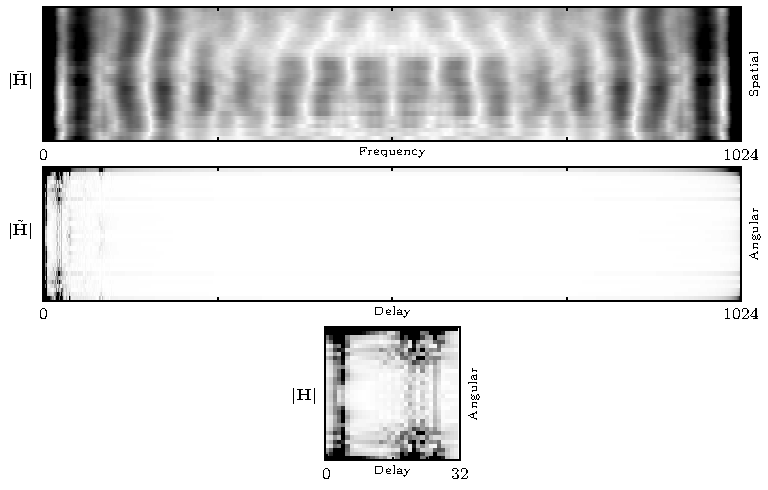
\includegraphics[width=.8\textwidth]{batch17_sample0_freqvsdel_truncatevsfull.pdf}
	\medskip
	\caption{Magnitude of spatial-frequency ($\bar{\mathbf H}$), angular-delay ($\tilde{\mathbf H}$), and truncated angular-delay ($\mathbf H$) CSI matrices for a single random channel.}
	\label{fig:freq-vs-delay}
\end{figure}

While the spatial-frequency representation, $\bar{\mathbf H}$, is used for beamforming at the transmitter, the number of non-zero elements is comparatively large (see Figure~\ref{fig:freq-vs-delay}, for example). In \cite{ref:csinet}, the authors choose to compress the \textbf{angular-delay} domain representation of CSI, $\tilde{\mathbf H}$.

Given the sparsity of the angular-delay matrices, many works using this basis choose to compress and feedback a truncated version of the CSI matrices, $\mathbf H \in \mathbb R^{R_d \times N_b}$. An illustrative example of this truncation can be seen at the bottom of Figure~\ref{fig:freq-vs-delay}.

\subsection{Bidirectional Reciprocity in FDD Networks}

As discussed in Section~\ref{sect:mimo_model}, the reciprocity of downlink and uplink channels is weak in FDD wireless networks when compared to TDD. Despite this, DL CSI estimation techniques have attempted to use uplink CSI to improve the quality of reconstructed downlink CSI at gNB. In \cite{ref:dualnet}, the authors demonstrate that the correlation between the magnitude of uplink and downlink CSI elements is strong, and they exploit the magnitude reciprocity with DualNet, a CNN autoencoder which feeds back encoded feedback for the magnitude of downlink CSI and decodes the feedback with the magnitude of uplink CSI as side information. The downlink phase is separately quantized and fed back to gNB via magnitude-dependent phase quantization (MDPQ). The authors demonstrate that exploiting bidirectional reciprocity can substantially improve CSI estimation accuracy.

\subsection{Temporal Coherence in Time-varying Channels}

\begin{figure}[htb] \centering 
  % 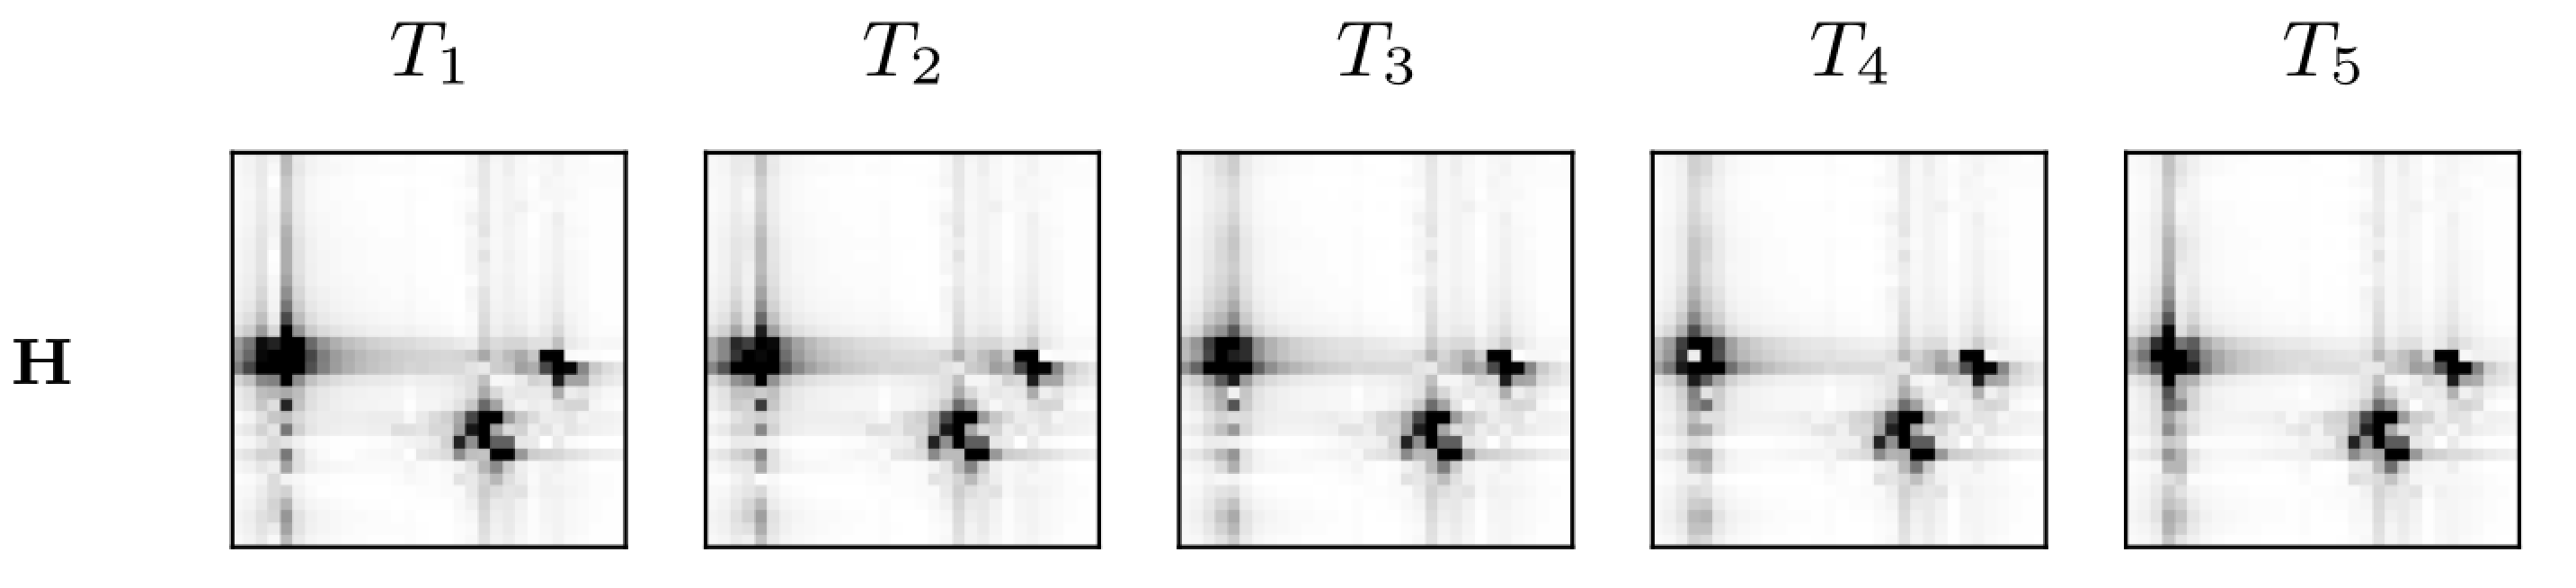
\includegraphics[width=0.9\linewidth]{batch0_csi_gt.png}
{
  \fontsize{10pt}{12pt}
  \def\svgwidth{1.0\columnwidth}
  \input{../images/batch0_csi_gt.pdf_tex}
}
  \caption{Ground truth CSI ($\mathbf H$) for five timeslots ($T_1$ through $T_5$) on one outdoor sample from the validation set.} 
  \label{fig:csi_img_gt} 
\end{figure}

Other works in channel state estimation exploit temporal coherence. The \emph{coherence time} of a channel is the amount of time channel estimate can be used before that estimate's SNR falls beneath a given threshold \cite{ref:Chopra2016ChannelAging}. Within this window of time ($\Delta T = T_i - T_{i-1}$), the correlation between CSI matrices $\mathbf H_{i}$ and $\mathbf H_{i-1}$ is high (see Figure~\ref{fig:csi_img_gt} for an illustrative example). Works exploiting temporal coherence use CSI matrices from previous timeslots to supplement subsequent estimates \cite{ref:Wang2019CsiNetLSTM}.

\subsection{Feedback Quantization}

To make CNNs practical for actual feedback transmission, authors have experimented with networks using entropy encoding for bit stream feedback \cite{ref:Yang2019DeepCMC} and networks with complex latent elements for IQ symbol feedback \cite{ref:Mashhadi2020AnalogDeepCMC}. These works incorporate entropy-based loss terms, and such rate-based optimization can achieve more compression at comparable distortion compared to autoencoders optimized via the non-regularized MSE. 

\section{Contributions}

This qualifying exam proposal details our attempts to use domain knowledge to enhance the performance and the efficiency of neural networks for CSI estimation. Section~\ref{chap:sph_norm} details our work in power-based normalization, which leverages CSI sparsity. Section ~\ref{chap:markovnet} describes our work in differntial encoding, which exploits temporal coherence of CSI. Section~\ref{chap:csinet_quant} describes our proposed work in trainable codewords, which incorporates data-adaptive quantization in the training process, and CSI entropy estimation, which establishes a compression bound for deep learning-based compressive feedback of CSI.